\chapter{Background and Problem Definition}
\label{chapter_background}

% **************************** Define Graphics Path **************************
\ifpdf
    \graphicspath{{Chapter3/Figs/Raster/}{Chapter3/Figs/PDF/}{Chapter3/Figs/}}
\else
    \graphicspath{{Chapter3/Figs/Vector/}{Chapter3/Figs/}}
\fi

This chapter establishes the terminology and basic formal definitions for this thesis and defines the problem of mining predictive episodes in a semi formal way (TODO: do that!).

\section{Episode Mining Background}
\label{sec_episodeMiningBackground}

While episodes were already intuitively defined and talked about in the previous chapters it is important to formally define episodes, since formal definitions are clear and unambiguous. This is important in order to define and explain mining objectives and techniques as well as algorithms that are used in this thesis. The rest of this section is divided as follows: %TODO: Subsection \ref{subsec_basicEpisodeDefinitions} formally introduces the concept of episodes, subsection \ref{subsec_episodeDiscovery} then follows  up with 

\subsection{Basic Definitions}
\label{subsec_basicEpisodeDefinitions}
As already mentioned, episodes are complex events whose basic building blocks are simple events. Note that  in order to make use of episodes we require that all simple events have a type and we have a finite, previously known event alphabet, that contains these types, which we refer to as $\Sigma$. We follow up with a formal definition:

\begin{mydef}
\label{def_episode}
\textbf{Episode} An episode (also sometimes called episode pattern or elementary episode) $\alpha$ of length $m$ (also called m-episode) is defined as a triple: $\alpha = (V_\alpha,{\leq}_{\alpha},g_\alpha)$ where $V_\alpha = \{v_1,...,v_m\}$ is a set of nodes, ${\leq}_{\alpha}$ is a partial order over $V_\alpha$ and $g_\alpha : V_\alpha \rightarrow \Sigma$ is a mapping that maps each node of $V_\alpha$ to an event type. \cite{mannila1995discovering}
\end{mydef}

Put more simply an episode is a multiset of event types, whose elements can be, but do not have to be ordered by a relation (${\leq}_{\alpha}$). Another way of putting it is that an episode is essentially a partially ordered sequence of events. Before we look at examples there are a two special types of episodes that need to be mentioned since they have received the most attention in the available literature. These are called serial and parallel episodes:

\begin{mydef}
\textbf{Serial Episode} An episode $\alpha = (V_\alpha,{\leq}_{\alpha},g_\alpha)$ is called a serial episode if ${\leq}_{\alpha}$ is a total order. \cite{mannila1995discovering}
\end{mydef}

\begin{mydef}
\textbf{Parallel Episode} An episode $\alpha = (V_\alpha,{\leq}_{\alpha},g_\alpha)$ is called a parallel episode if ${\leq}_{\alpha} = \emptyset$, in other words if there is no ordering imposed on $V_\alpha$ at all. \cite{mannila1995discovering}
\end{mydef}

Essentially, serial episodes are sequences, while parallel episodes are multisets. Figure \ref{fig_exampleEpisodes} visualizes example episodes in the same way that we have visualized episodes in earlier chapters, namely as directed acyclic graphs (DAG).

\begin{figure}[h]
	\centering
  	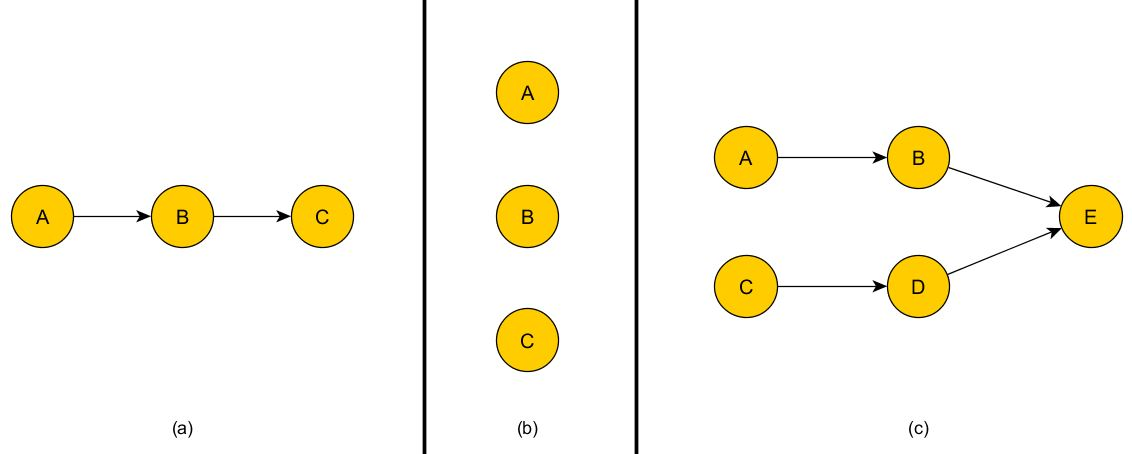
\includegraphics[width=\textwidth]{exampleEpisodes}
	\caption{An example of different episodes: (a) - a serial episode, (b) - a parallel episode, (c) - an elementary (composite) episode}
	\label{fig_exampleEpisodes}
\end{figure}

%\begin{figure}[H]
%\centering
%\begin{tabular}{c|c|c}
%\begin{subfigure}{.3\textwidth}
%  \centering
%  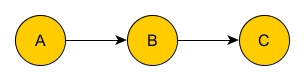
\includegraphics[width=\linewidth]{exampleSerialEpisode}
%  \caption{A serial episode}
%  \label{fig:sub1}
%\end{subfigure}%
%&
%\begin{subfigure}{.3\textwidth}
%  \centering
%  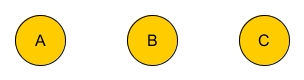
\includegraphics[width=\linewidth]{exampleParallelEpisode}
%  \caption{A parallel episode}
%  \label{fig:sub2}
%\end{subfigure}
%&
%\begin{subfigure}{.3\textwidth}
%  \centering
%  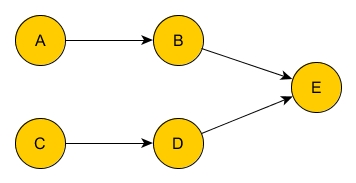
\includegraphics[width=\linewidth]{exampleCompositeEpisode}
%  \caption{An elementary (composite) episode}
%  \label{fig:sub3}
%\end{subfigure}
%\end{tabular}
%\caption{Different example episodes visualized as directed acyclic graphs}
%\label{fig_exampleEpisodes}
%
%\end{figure}

In fact each episode can be formally transformed to a DAG using the following simple procedure: Given an Episode $\alpha = (V_\alpha,{\leq}_{\alpha},g_\alpha)$, create the corresponding DAG $G = (V,E)$ by executing the following:

\begin{enumerate}
	\item For each $v \in V_\alpha$ add $v$ to $V$ and label $v$ with $g_\alpha (v)$
	\item For each pair $v,w \in V_\alpha$ where $v \, {\leq}_{\alpha} \, w $ add edge $(v,w)$ to $E$
\end{enumerate}

The original paper by Manilla et.al. \cite{mannila1995discovering} also introduces the notion of composite episodes. We repeat the definition here:

\begin{mydef}
\label{def_compositeEpisodes}
\textbf{Composite Episode} An episode $\alpha = (V_\alpha,{\leq}_{\alpha},g_\alpha)$ is called a composite episode if $g_\alpha : V_\alpha \rightarrow \Sigma \cup C^*$, where $C^*$ is the set of all composite episodes. \cite{mannila1995discovering}
\end{mydef}

This recursive definition of composite episodes may be confusing at first, since it is formulated very compactly. A slightly more clear way to look at it is the following:\\
A composite episode is either:
\begin{itemize}
	\item A single event (An elementary episode of size 1).
	\item A serial composition of two composite episodes
	\item A parallel composition of two composite episodes
\end{itemize}

This definition has the advantage that any elementary episode can be represented as a composite episode which is exclusively a serial or parallel composition of serial, parallel or composite subepisodes (see definition \ref{def_subEpisode}). Note that composite episodes are not more expressive than elementary episodes as defined in definition \ref{def_episode}, it is just a recursive way of defining episodes. \\
Interestingly, there are other parts of the related work that use the term \textit{composite episodes} but deviate from definition \ref{def_compositeEpisodes}. For example Baathorn et. al. propose a method for finding composite episodes \cite{bathoorn2007finding}. However they define composite episodes as a sequence of parallel episodes, which is more restrictive than the original definition. Also Baumgarten et. al. use this definition \cite{baumgarten2003tree} when they present an approach to mine descriptive composite episodes. Note that not all elementary episodes can be represented as sequences of parallel episode. A simple example shown in figure \ref{fig_notSequenceOfSet} illustrates this. If the presented episode were to be represented as a sequence of parallel episodes obviously $A$ and $B$ would have to be in different parallel episodes in order to fulfill the requirement that $B$ must be after $C$. After that the problem is that it is impossible to assign $C$ to any of those sets. If it gets assigned to the same parallel episode set as $A$ then this would prohibit $A$ and $B$ occurring first followed by $C$, which is allowed in the original definition. Likewise if $C$ gets assigned to the same parallel episode as $B$ then that eliminates the possibility of $C$ occurring before $A$ and $B$, which once again was allowed in the elementary episode. In this thesis we will stick to the original definition as presented in definition \ref{def_compositeEpisodes}. \newline

\begin{figure}[h]
	\centering
  	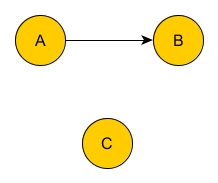
\includegraphics[width=0.3\textwidth]{notSequenceOfSet}
	\caption{An elementary episode that can not be represented as a sequence of parallel episodes}
	\label{fig_notSequenceOfSet}
\end{figure}

If we want to quickly denote simple episodes formally without drawing a DAG, we will use $\rightarrow$ as the sequence (ordering) operator. To show that there is no order specified between two nodes we use $\|$ as the parallel operator. For example $(A \, \| \, B ) \rightarrow C$ denotes a composite episode of length 3, which specifies that it does not matter in which order $A$ or $B$ occur, but $C$ must occur after both $A$ and $B$. If we want to discuss more complex episodes we will visualize them graphically like in the previous figures \newline  
The notion of sub- and superpatterns, which is very important for most pattern mining applications also applies to episodes, as shown in the next definition.

\begin{mydef}
\label{def_subEpisode}
\textbf{Subepisode} An episode $\beta = (V_\beta,{\leq}_{\beta},g_\beta)$ is said to be a subepisode of episode $\alpha = (V_\alpha,{\leq}_{\alpha},g_\alpha)$ if all of the following conditions hold:
\begin{enumerate}
	\item The nodes of $\beta$ are a subset of the nodes of $\alpha$: \\
	$V_\beta \subseteq V_\alpha$
	\item All nodes of $\beta$ are assigned to the same event type as their corresponding nodes in $\alpha$:\\
	 $\forall v \in V_\beta \; : \; g_{\beta}(v) = g_\alpha (v) $
	\item The ordering in $\alpha$ is at least as strict as the ordering in $\beta$:\\
	$\forall v,w \in V_\beta \, , v \, {\leq}_{\beta} \, w \; : \; v \, {\leq}_{\alpha} \, w$
\end{enumerate}
In this context we also refer to $\alpha$ as the superepisode of $\beta$. \cite{mannila1995discovering,laxman2007fast}.
\end{mydef}

It is important to note that in the original definition of sub- and superepisodes by Mannila et. al. \cite{mannila1995discovering}, the first property of the above definition was actually defined as $V_\beta \subset V_\alpha$, which implies that subepisodes would always have to consist of at least one less node than their superepisodes. This definition was changed by Laxman et. al. \cite{laxman2007fast} to allow set equality as well. The implications of this change are that parallel episodes like $A \| B$ are now subepisodes of their serial counterparts of the same length $A \rightarrow B$. In this thesis we stick to the definition that allows set equality between super- and subepisodes. In both cases however subepisodes may relax the ordering specified in their superepisodes. For example if given the serial episode $\alpha =( A \rightarrow B \rightarrow C )$, not only $A \rightarrow B$ is a subepisode of $\alpha$ but also $A \| B$. \\
So far we have talked a lot about episode patterns but we have not yet talked about the detection such episodes in data. It is helpful to think of the episode patterns we have defined above as templates for concrete occurrences. In order to define what we mean by an episode occurrence, we first need to formally introduce the notion of an event sequence.

\begin{mydef}
\label{def_eventSequence}
\textbf{Event sequence} An event sequence is defined as an ordered list of tuples $S = [ (T_1,t_1),..., (T_n,t_n) ] $ where $T_i \in \Sigma$ is the event type of the i-th event and $t_i \in \mathbb{N}^+$ is the timestamp of the i-th event. The sequence is ordered according to the timestamps, which means that $\forall i,j \in {1,...,n} \; i<j \implies t_i \leq t_j$. \cite{mannila1997discovery} %TODO: talk about time equality
\end{mydef}

Note that it is allowed for two or more consecutive elements in a sequence to have the same timestamp. This is necessary in order to allow for multiple events to occur at the same time. The ordering of events with the same timestamp is not further specified and irrelevant in most cases. Another way to define such sequences is to define them as sequences of event sets in which consecutive event sets must all have different timestamps and events that occur simultaneously are part of the same set \cite{bathoorn2007finding}. Definitions from other authors explicitly prohibit two events happening at the same time \cite{baumgarten2003tree}. Which definition is appropriate depends on the context, for this thesis we will stick with definition \ref{def_eventSequence}. \\
Given the notion of an event sequence we can now define episode occurrences:

\begin{mydef}
\label{def_episodeOccurrence}
\textbf{Episode Occurrence} An event episode $\alpha = (V_\alpha,{\leq}_{\alpha},g_\alpha)$ is said to occur in a sequence $S$ if events of the types that the nodes in $V_\alpha$ are mapped to by $g_\alpha$, occur in $S$ in the same order that they occur in the episode. More formally if we are given a sequence of events $S=[(T_1,t_1),...,(T_n,t_n)]$ we can define an occurrence of $\alpha$ as an injective Map $h:V_\alpha \rightarrow \{1,...,n\}$, where $g_\alpha (v) = T_{h(v)}$ and $\forall \, v,w \in V\alpha : v \;{\leq}_{E}\; w \implies t_{h(v)} \le t_{h(w)}$ holds. \cite{mannila1995discovering}
\end{mydef}

An example of an episode pattern, a sequence and two occurrences is visualized in figure \ref{fig_occurrenceExample}.

\begin{figure}[h]
	\centering
  	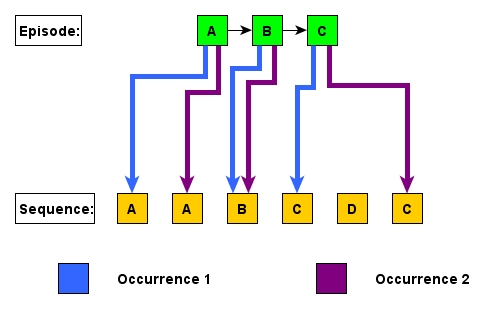
\includegraphics[width=\textwidth]{occurrenceExample}
	\caption{A visualization of the concept of episode occurrences in an event sequence. The episode pattern is drawn in green, the sequence in yellow. An occurrence is defined as a mapping from the nodes of the pattern to events in the sequence (see definition \ref{def_episodeOccurrence}). Thus the occurrences are visualized as arrows of different colors (blue and purple). }
	\label{fig_occurrenceExample}
\end{figure}


\subsection{Episode Discovery and general Mining Algorithm}
\label{subsec_episodeDiscovery}
When discovering episodes in a sequence one is usually interested in those episodes that occur frequently, meaning more often than a user defined threshold. This is similar to all the different kinds of pattern mining algorithms, such as the apriori algorithm for finding frequent itemsets \cite{agrawal1994fast}. A general algorithm for mining the episodes occurring frequently in a sequence is given in algorithm \ref{alg_generalEpisodeMining}. The algorithm is very alike the basic apriori algorithms, since it uses a level-wise, breadth first search by first identifying all frequent episodes of a certain length $i$ and then uses these frequent episodes to generate candidates (possibly frequent episodes) of length $i+1$. In order for this to be correct, episode frequency must follow the apriori principle \cite{agrawal1994fast}, which formally means that if an episode is frequent, all its subepisodes must be frequent as well. Intuitively one would assume that this is always true for episodes but strictly speaking this depends on the definition of episode frequency. However, any frequency definition of episodes that does not satisfy the apriori principle would be highly questionable to say the least, since this would eliminate the possibility of an efficient candidate generation that prunes those episodes which have infrequent subepisodes. To the best of our knowledge all frequency definitions proposed in the literature satisfy the apriori principle.\newline

\begin{algorithm}[H]
  \caption{General mining algorithm for frequent episodes
    \label{alg_generalEpisodeMining}}
  \begin{algorithmic}[1]
    \Statex
    \Function{EpisodeMining}{}
      \Let{$C_i$}{Episodes of Size 1} 
      \Let{$freq$}{$\emptyset$}
      \Let{$i$}{$1$}
      \While{$C_i \neq \emptyset$}
      	\State Count frequencies of each Episode $E \in C_i$
        \Let{$L_i$}{ $\{ E \mid E \in C_i \land C_i \; is\; frequent\}$}
        \Let{$freq$}{$freq \cup L_i$}
        \Let{$C_{i+1}$}{Generate Episode Candidates of length $i+1$ from $L_i$}
        \Let{$i$}{$i+1$}
      \EndWhile
      \State \Return{$freq$}
    \EndFunction
  \end{algorithmic}
\end{algorithm}


In summary, the general mining algorithm for frequent episodes requires:

\begin{itemize}
	\item A definition of episode frequency, that does not violate the apriori principle
	\item An algorithm for counting episode frequency (of concrete candidates) according to this definition
	\item An algorithm to generate candidate episodes
\end{itemize}

It may be a bit confusing that we need a definition of episode frequency for such a mining algorithm. Since we have already defined what an occurrence of an episode looks like it would seem that counting all occurrences of an episode would yield its frequency. While this is a possible definition of frequency, it is important to note that finding all occurrences of an episode within a sequence is neither practical nor useful. An example will demonstrate the problem with this. Consider the simple serial episode $A \rightarrow B$ and a sequence of length $2\cdot n$ which repeats the subsequence $(A,B)$ $n$ times. One quickly realizes that the number of episode occurrences is very large due to the possibility of overlapping episode occurrences. In this particular case there are already $ \frac{n \cdot (n+1)}{2}$ possible occurrences. This number swiftly increases with the size of the episode pattern, since it introduces more potential overlappings. Naturally the number of possible parallel and composite episode occurrences is even larger, since they are less restrictive in the order of the events. Additionally, such a frequency definition would violate the apriori principle, since subepisodes can have less occurrences than their superepisodes. Consider the example sequence $[A,B,C,A,B,C]$ (timestamp values are left out). In this sequence there are 3 distinct occurences for the episode $A \rightarrow B$ and four distinct occurrences for its superepisode $A \rightarrow B \rightarrow C$. These detrimental effects of this naive frequency definition are nicely summarized by Laxman et. al. in a paper presenting the non-overlapped frequency definition \cite{laxman2007fast}. \newline
This leads to various frequency definitions of episodes in the literature, which will be dealt with in subsections \ref{subsec_windowBased} and \ref{subsec_otherFrequency}. Each frequency definition comes with its own frequency counting algorithm. The procedure for generating candidates is independent of the frequency definition and is presented in \ref{subsec_candidateGen}. \newline
%The first two definitions, which we will refer to as window based frequency and minimal occurance based frequency, are mentioned by Zimmermann, when he presents his method for synthetic episode generation \cite{zimmermann2012generating}, but were originally conceived in (TODO: include original sources). We refer to the third definition as the non-overlapping occurrence based Frequency which was suggested by Laxman et al. \cite{laxman2007fast}.


\subsection{Window based frequency}
\label{subsec_windowBased}
To the best of our knowledge the window based frequency was the first frequency definition for episodes to gain general popularity. It was conceived by Mannila et. al. \cite{mannila1995discovering}, although the frequency counting algorithms were only mentioned in text form. The same authors  specified the algorithms in a later paper \cite{mannila1997discovery}, which acts as the primary source for the overview given in this subsection. In order to define the window based frequency we first need the notion of a time window: 

\begin{mydef}
\textbf{Time Window} Given a sequence of events $S$ we define the Time Window $W(S,q,r)$ with $q,r \in \mathbb{N}^+$ and $q < r$ as the ordered subsequence of $S$ that includes all events of the annotated event stream $S$ that have a timestamp $t$ where $q \leq t\leq r$. We call $w = r-q+1$ the size of Window $W$.
\end{mydef}

An example of how windows of a fixed size are located in a sequence of events is presented in figure \ref{fig_windowBasedFrequency}.

\begin{figure}[h]
	\centering
  	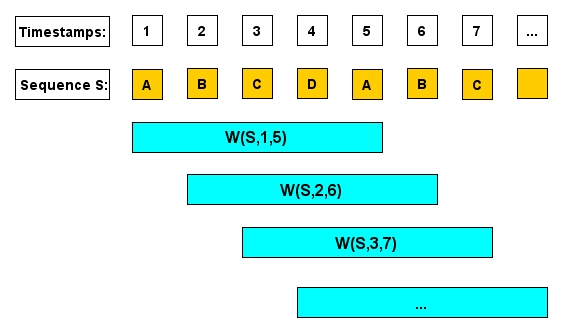
\includegraphics[width=\textwidth]{windowBasedFrequency}
	\caption{Different time windows of size 5 in an event sequence.}
	\label{fig_windowBasedFrequency}
\end{figure}


\begin{mydef}
\textbf{Episode Frequency - Window based Definition} Given a sequence of events $S$, a fixed window size of $w$ and an episode $\alpha$, we define the window based frequency $w\_freq(\alpha )$ as the number of windows $W$ with size $w$ of $S$ in which $\alpha$ occurs: $w\_freq(\alpha ) = |\,\{W(S,q,r) \mid r-q+1 = w \land \alpha \;occurs\; in\; W \}\,|$. %TODO: incorporate sequence bounds and number of windows
\end{mydef}


For example given the sequence visualized in figure \ref{fig_windowBasedFrequency} $A \rightarrow B \rightarrow C$ occurs in windows $W(S,1,5)$ and $W(S,3,7)$. \newline 
This definition can be confusing at first since it is intended that episode occurrences that are comprised of the exact same events count just as many times as there are windows in which the events appear. In the previously mentioned example, we can find the episode $C \rightarrow D$ in the consecutive windows $W(S,1,5)$, $W(S,2,6)$ and $W(S,3,7)$, which means we will get a frequency of $3$ just for the two events $(3,C)$ and $(4,D)$. This effect obviously increases with the window size. Note that for each episode $\alpha$ we only count one occurrence per window $W$, no matter how many occurrences of $\alpha$ there are in $W$.\newline
When determining the window based frequency the naive approach would be to check each window of the sequence separately. Since the windows are adjacent there is a better approach, which makes it possible to only iterate over the sequence once and determine the window based frequency for each candidate episode. Most papers focus purely on parallel and serial episodes and do not give an algorithm for composite episodes. The algorithms to determine the window based frequency of serial and parallel episodes can be looked up in the appendix \ref{app_freqCounting}.
There is a notable absence of frequency counting algorithms for elementary (composite) episodes in literature. Mannila et. al. claim that each composite episode can be broken down into partial episodes, which are serial and/or parallel \cite{mannila1997discovery}. However they neither specify an algorithm for breaking down composite episodes into purely serial and parallel parts, nor do they specify a frequency counting algorithm for composite episodes. Subsequent research, such as alternate frequency definitions and counting algorithms has also mainly focused on parallel and serial episodes. If composite episodes have been studied they were usually studied in the above mentioned, more restrictive form of sequences of parallel episodes. \newline

\subsection{Other frequency definitions}
\label{subsec_otherFrequency}

In this subsection we briefly present alternative frequency definitions without specifying counting algorithms. For the exact algorithms we refer the reader to the respective papers. \newline
Most alternative definitions tried to move away from the ideas of fixed windows and tried to improve the performance of the counting algorithms. \\
\\
\textbf{Minimal Occurrence Based Frequency Definition} \newline
The first alternate definition does uses the concept of minimal occurrences:

\begin{mydef}
\textbf{Minimal Occurrence} An event episode $\alpha$ is said to occur minimally in a window $W(S,q,r)$ if $\alpha$ occurs in $W$ and there is no subwindow of $W$ in which $\alpha$ also occurs. %(TODO: define subwindow)
\end{mydef}

\begin{mydef}
\textbf{Episode Frequency - Minimal Occurrence based Definition} Given a sequence of events $S$ and an Episode $\alpha$, we define the minimal occurrence based frequency $mo\_freq(\alpha )$ as the number of minimal occurrences of $\alpha$ in $S$. TODO: find and cite the original source
\end{mydef}

The second alternative definition introduces the concept of non-overlapping occurrences:

\begin{mydef}
\textbf{Non-Overlapping Occurrences} Given a m-Episode $\alpha = (V_\alpha,{\leq}_{\alpha},g_\alpha)$ where $V_\alpha = \{v_1,...,v_m\}$, two occurrences if all timestamps of one of the occurrences are bigger than all the timestamps of the other occurrence. Formally two occurrences $h_1$ and $h_2$ of $\alpha$ are non-overlapped if either:
\begin{itemize}
	\item $\forall \, v_j \in V_\alpha : h_2(v_1)>h_1(v_j)$ or 
	\item $\forall \, v_j \in V_\alpha : h_1(v_1)>h_2(v_j)$
\end{itemize}
A set of occurrences is non-overlapping if every pair of occurrences in it is non-overlapped \cite{laxman2007fast}.
\end{mydef}

An example scenario visualizing overlapping and non-overlapping occurrences is visualized in figure \ref{fig_nonOverlappingExample}.


\begin{figure}[h]
	\centering
  	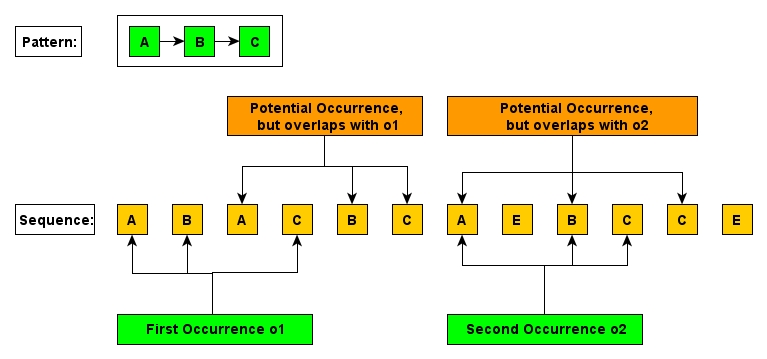
\includegraphics[width=\textwidth]{nonOverlappingExample}
	\caption{An example sequence that shows how occurrences of episode patterns can overlap. Two non-overlapping occurrences are colored in green, whereas the orange occurrences would overlap with one of the green occurrences.}
	\label{fig_nonOverlappingExample}
\end{figure}

This leads to the Definition:

\begin{mydef}
\textbf{Episode Frequency - Non-Overlapping Occurrences based Definition} Given a seqeunce of events $S$ and an Episode $\alpha$, we define the non-overlapping occurrence based frequency $noo\_freq(\alpha )$ as cardinality of the largest set of non-overlapped occurrences of $\alpha$ in $S$ \cite{laxman2007fast}.
\end{mydef}


When looking at these definitions in comparison to the window based frequency definition it is not clear whether any of these is always superior to or more useful than the other since they have different properties. We mention them briefly:

\begin{itemize}
	\item As already mentioned the window based frequency counts an episode occurrence that is comprised of the same events in multiple windows. This might especially distort the count if the window size is high and the events in the episode happen with minimal delay between them.
	\item The minimal occurrence based definition of frequency does not suffer from the problem of the previous point
	\item The window based definition has the advantage that it already incorporates a fixed size during which episodes may occur, meaning there can not be episodes that stretch over a time period larger than the fixed window size $w$. This might be beneficial for potential algorithms, since it reduces the search space for episodes. On top of that it is also closer to reality, since in many domains episodes happen within a small time window \cite{generatingEpisodeDatasets}.
	\item The non-overlapping occurrence based frequency offers the fastest counting algorithm of all three definitions. However when incorporating expiry times for serial episodes it looses this advantage. Additionally previous literature has not yet identified an efficient algorithm to count non-overlapped occurrences of parallel episodes with expiry times. 
\end{itemize}

\subsection{Candidate Generation}
\label{subsec_candidateGen}
Most previous work generates candidates for serial and parallel episodes separately, using a levelwise approach for both cases. The candidate generation procedure presented below was originally specified by Manila et. al. \cite{mannila1997discovery}. A more detailed explanation can be found in Laxman's PHD thesis \cite{laxman2006discovering}. \newline
We first consider the case for parallel episodes. Given $F_k$ as the set of all frequent parallel episodes of length $k$ we can generate the candidate parallel episodes $C_{k+1}$ of length $k+1$ by doing the following:

\begin{enumerate}
	\item Represent each candidate $\alpha \in F_k$ as a lexicographically sorted array of length $k$.
	\item For each unordered pair $(\alpha , \beta )$, $\alpha ,\beta \in F_k$ where $\alpha$ and $\beta$ share the same first $k-1$ nodes, generate candidate $\gamma$ by copying $\alpha$ and appending $\beta [k]$.
\end{enumerate}

For example the two frequent parallel episodes $A \| A \| B$ and $A \| A \| C$ will generate the candidate $A \| A \| C \| D$. \newline
The same procedure can be applied to serial episodes, except that
\begin{itemize}
	\item we do not order lexicographically, instead the serial episodes remain in the array in their natural order
	\item each pair $(\alpha , \beta )$ with the same properties as above now generates two candidates:
	\begin{itemize}
		\item $\gamma{_1}$ by copying $\alpha$ and appending $\beta [k]$.
		\item $\gamma{_2}$ by copying $\beta$ and appending $\alpha [k]$.
	\end{itemize}
\end{itemize}

Thus the two frequent serial episodes $A \rightarrow A \rightarrow B$ and $A \rightarrow A \rightarrow C$ will now generate the two candidates $A \rightarrow A \rightarrow B \rightarrow C$ and $A \rightarrow A \rightarrow C \rightarrow B$. \newline
Since the mining of composite episodes has not received much attention, it is unsurprising that there little related work that mentions candidate generation strategies for these general types of episodes (TODO: refer to later chapter, since I will do that). For a more strict definition of composite episodes which only includes sequences of parallel episodes, Baumgarten et. al. use a tree growth strategy to generate candidates for composite episodes \cite{baumgarten2003tree}. %TODO: expand this subsection if needed

\section{Problem Definition}
As already mentioned before the problem to be tackled in this thesis is the prediction of future events in data streams using episodes. The approaches shall have the following properties:

\begin{itemize}
	\item \textbf{Local and fast prediction:} We do not focus on long term trends or on predictions of special values at fixed times (for example daily closing values of stocks), but instead aim to give predictions about the near future given the current state of the stream.
	\item \textbf{Usage of an Annotated Event Stream} Most forecasting methods (as reviewed in TODO) focus on regression, meaning the predictions of numerical values. In contrast to this we work on annotated event streams, meaning we deal with a stream of events, which have predefined types (which is necessary to discover episodes) and we aim to predict the occurrences of events of certain types.
\end{itemize}

Since a lot of basic streams are numeric in nature we define:

\begin{mydef}
\textbf{Low Level Event Stream} A Low Level Event stream is defined as a (possibly infinite or constantly updating) sequence: $LLES = [v_1,v_2,...]$ where each $v_i$ has the form of a tuple: $t_i = (t_i,v_{i1},v_{i2},...,v_{in})$ where $t_i \in \mathbb{N}$ is the timestamp of tuple $i$ and $v_{ij}$ is the j-th value of the i-th tuple. The datatypes of the values in the tuple depend on the concrete domain or stream, so they are not further specified. Common types are numerical, categorical or string values. The Low Level Event Stream is ordered by the timestamp values, but events are allowed to occur at the same time. Formally this means: $T_i \leq T_j \implies i \leq j$. 
\end{mydef}

We refer to the streams that we perform the suggested mining approaches on as Annotated Event Streams:

\begin{mydef}
\textbf{Annotated Event Stream} An Annotated Event Stream is defined as a (possibly infinite or constantly updating) sequence: $AES = [ (T_1,t_1),(T_2,t_2),... ] $ where $T_i \in \Sigma$ is the event type of the i-th event and $t_i \in \mathbb{N}^+$ is the timestamp of the i-th event. The sequence is ordered according to the timestamps, which means that $\forall i,j \in {1,...,n} \; i<j \implies t_i \leq t_j$.
\end{mydef}

Note that this definition is essentially the same as definiton \ref{def_eventSequence}, which defines event sequences. The only difference is that in an Annotated Event Stream we allow for new events to constantly come in, which makes the sequence possibly infinite.
If the original underlying data source is a low level event stream it needs to be transformed to an annotated event stream, which can be done via a transformation procedure:

\begin{mydef}
\textbf{Tranformation Procedure} A transformation procedure is a mapping $f$ that takes a low level event stream $LLES$ as an input and outputs an annotated event stream $AES$ as well as the corresponding event aphabet $\Sigma$.
\end{mydef}

Note that the selection or development of the transformation procedure is extremely important for the success of the subsequent mining of the annotated event stream. If the annotated events that are generated are largely meaningless due to a suboptimal transformation it is unlikely that the mining process will discover episodes that are helpful to predict occurrences of the desired events. 
TODO: Aggregation, discretization
If the low level annotated stream is processed in an online scenario, it is necessary to also do the transformation in an online way, which imposes additional restrictions on the transformation process (TODO: exmplain those).

Given an annotated event stream $AES$ it is the goal of this thesis to develop algorithms that will build predictive models:

\begin{mydef}
\label{def_predictiveModel}
\textbf{Predictive Model} A predictive model for $M(T)$, $T \in Sigma$ is a model that if given the current state of an annotated event stream will output a binary value in the following:
\begin{itemize}
	\item $1$ if the model expects an event of type $T$ to occur in the stream in the near future
	\item 0 otherwise.
\end{itemize} 
\end{mydef}

Definition \ref{def_predictiveModel} purposefully remains rather general and thus vague, since a predictive model can naturally function in many ways. Thus some of the key points, such as what is the state of a stream and what exactly does the term "near future" mean mathematically remain unspecified here and instead will be specified by the concrete algorithms. 
Nevertheless one should note that in most streaming scenarios we cannot store the whole stream, meaning it is impractical for a model to demand that the current state of the stream is defined by its entire history. Likewise a model may define that the "near future" means an extremely long time, thus most likely making the model correct if it simply outputs $1$ every time, however such a model is obviously not very useful.